% !TeX root = mos-en.tex

%%%%%%%%%%%%%%%%%%%%%%%%%%%%%%%%%%%%%%%%%%%%%%%%%%%%%%%%%%%%%%%%

\begin{prob}{Should you sample with or without replacement?\annotate{D,S}}
Urn $A$ contains $2$ red balls and $1$ green ball, and urn $B$ contains $101$ red balls and $100$ green balls. An urn is chosen at random and two balls are randomly drawn \emph{from the selected urn}. You win if you correctly identify whether the selected urn was $A$ or $B$.

Which of the following rules gives you the highest probability of winning?

\que{1} The first ball is replaced before the second drawing.

\que{2} The first ball is not replaced before the second drawing.

\que{3} After the first ball is drawn you can decide whether it will be replaced or not.

\textbf{Hint:} When computing probabilities:
\[
\disfrac{101}{201}\approx \disfrac{100}{201} \approx \disfrac{100}{200} \approx \disfrac{1}{2}\,.
\]
\end{prob}

\vspace{-5ex}

\solution{}

There are four outcomes which we denote by $RR, RG, GR, GG$. For each rule compute the conditional probabilities of the four outcomes given that urn $A$ or urn $B$ was selected initially. These multiply by $1/2$ to take into account the random selection of the urn.

\ans{1} Drawing with replacement:
\[
\renewcommand*{\arraystretch}{1.5}
\begin{array}{lcccc}
P(RR|A) &=& \frac{2}{3} \cdot \frac{2}{3} &=& \frac{4}{9}\\
P(RR|B) &=& \frac{1}{2} \cdot \frac{1}{2} &=& \frac{1}{4}\\
\hline
P(RG|A) &=& \frac{2}{3} \cdot \frac{1}{3} &=& \frac{2}{9}\\
P(RG|B) &=& \frac{1}{2} \cdot \frac{1}{2} &=& \frac{1}{4}\\
\hline
P(GR|A) &=& \frac{1}{3} \cdot \frac{2}{3} &=& \frac{2}{9}\\
P(GR|B) &=& \frac{1}{2} \cdot \frac{1}{2} &=& \frac{1}{4}\\
\hline
P(GG|A) &=& \frac{1}{3} \cdot \frac{1}{3} &=& \frac{1}{9}\\
P(GG|B) &=& \frac{1}{2} \cdot \frac{1}{2} &=& \frac{1}{4}\end{array}
\]
If the outcome is $RR$ there is a higher probability that urn $A$ was selected ($4/9$) than that urn $B$ was selected ($1/4$); otherwise, there is a higher probability that urn $B$ was selected:
\[
P(\textsf{winning})=\frac{1}{2}\left(\frac{4}{9} + \frac{1}{4}+ \frac{1}{4}+ \frac{1}{4}\right)=\disfrac{43}{72}\approx 0.5972\,.
\]

\ans{2} Drawing without replacement:
\[
\renewcommand*{\arraystretch}{1.5}
\begin{array}{lcccc}
P(RR|A) &=& \frac{2}{3} \cdot \frac{1}{2} &=& \frac{1}{3}\\
P(RR|B) &=& \frac{1}{2} \cdot \frac{1}{2} &=& \frac{1}{4}\\
\hline
P(RG|A) &=& \frac{2}{3} \cdot \frac{1}{2} &=& \frac{1}{3}\\
P(RG|B) &=& \frac{1}{2} \cdot \frac{1}{2} &=& \frac{1}{4}\\
\hline
P(GR|A) &=& \frac{1}{3} \cdot 1 &=& \frac{1}{3}\\
P(GR|B) &=& \frac{1}{2} \cdot \frac{1}{2} &=& \frac{1}{4}\\
\hline
P(GG|A) &=& \frac{1}{3} \cdot 0 &=& 0\\
P(GG|B) &=& \frac{1}{2} \cdot \frac{1}{2} &=& \frac{1}{4}
\end{array}
\]
If the outcome is $GG$ there is (of course!) a higher probability that urn $B$ was selected than that urn $A$ was selected; otherwise, there is a higher probability that urn $A$ was selected. The probability of winning is:
\[
P(\textsf{win})=\frac{1}{2}\left(\frac{1}{3} + \frac{1}{3}+ \frac{1}{3}+ \frac{1}{4}\right)=\frac{5}{8}=0.6250\,,
\]
which is greater than the probability of winning when sampling with replacement.

\ans{3} The decision is based on the outcome of the first draw.

If the first drawing is from urn $A$ the probabilities must be conditioned on the decision to sample with or without replacement. Drawing first from urn $B$ does not affect the probabilities because of the approximation in the hint.
\[
\renewcommand*{\arraystretch}{1.5}
\begin{array}{lcccc}
P(RR|A,w) &=& \frac{2}{3} \cdot \frac{2}{3} &=& \frac{4}{9}\\
P(RR|A,w/o) &=& \frac{2}{3} \cdot \frac{1}{2} &=& \frac{1}{3}\\
P(RR|B) &=& \frac{1}{2} \cdot \frac{1}{2} &=& \frac{1}{4}\\
\hline
P(RG|A,w) &=& \frac{2}{3} \cdot \frac{1}{3} &=& \frac{2}{9}\\
P(RG|A,w/o) &=& \frac{2}{3} \cdot \frac{1}{2} &=& \frac{1}{3}\\
P(RG|B) &=& \frac{1}{2} \cdot \frac{1}{2} &=& \frac{1}{4}\\
\hline
%\end{array}
%\]
%\[
%\renewcommand*{\arraystretch}{1.5}
%\begin{array}{lcccc}
P(GR|A,w) &=& \frac{1}{3} \cdot \frac{2}{3} &=& \frac{2}{9}\\
P(GR|A,w/o) &=& \frac{1}{3} \cdot 1 &=& \frac{1}{3}\\
P(GR|B) &=& \frac{1}{2} \cdot \frac{1}{2} &=& \frac{1}{4}\\
\hline
P(GG|A,w) &=& \frac{1}{3} \cdot \frac{1}{3} &=& \frac{1}{9}\\
P(GG|A,w/o) &=& \frac{1}{3} \cdot 0 &=&0\\
P(GG|B) &=& \frac{1}{2} \cdot \frac{1}{2} &=& \frac{1}{4}\\\end{array}
\]
If a red ball is drawn first then $\frac{4}{9}>\frac{1}{4}$ and $\frac{2}{9}<\frac{1}{4}$ with replacement, whereas $\frac{1}{3}>\frac{1}{4}$ and $\frac{1}{3}>\frac{1}{4}$ without replacement, so the second ball can help identify the urn only if the drawing is done \emph{with} replacement: urn $A$ if red, urn $B$ if green. Choose the draw with replacement:
\[
P(\textsf{winning if red first})=\frac{1}{2}\left(\frac{4}{9}+\frac{1}{4}\right)=\frac{25}{72}\,.
\]
If a green ball is drawn first then $\frac{2}{9}<\frac{1}{4}$ and $\frac{1}{9}<\frac{1}{4}$ with replacement, whereas $\frac{1}{3}>\frac{1}{4}$ and $0<\frac{1}{4}$ without replacement, so the second ball can help identify the urn only if the drawing is done \emph{without} replacement: urn $A$ if red, urn $B$ if green. Choose the draw without replacement:
\[
P(\textsf{winning if green first})=\frac{1}{2}\left(\frac{1}{3}+\frac{1}{4}\right)=\frac{7}{24}\,.
\]
The total probability of winning is:
\[
P(\textsf{winning})=\frac{25}{72} + \frac{7}{24}=\frac{23}{36}\approx 0.6389\,.
\]
The highest probability of winning is obtained when the decision to draw with or without replacement depends on the result of the first draw.

\textbf{Simulation}
\begin{verbatim}
With replacement:
Expectation of winning = 0.5972
Average wins           = 0.5976
Without replacement:
Expectation of winning = 0.6250
Average wins           = 0.6207
Decide after first draw:
Expectation of winning = 0.6389
Average wins           = 0.6379
\end{verbatim}


%%%%%%%%%%%%%%%%%%%%%%%%%%%%%%%%%%%%%%%%%%%%%%%%%%%%%%%%%%%%%


\begin{prob}{The ballot box\annotate{S}}
In an election there are two candidates $A$ and $B$.  $A$ receives $a$ votes and $B$ receives $b$ votes, $a>b$. The votes are counted one-by-one and the running totals $(a_i,b_i), 1\leq i \leq a+b$ are updated as each vote is counted. What is the probability that for at least one $i$, $a_i=b_i$?

\que{1} Solve for $a=3, b=2$ by listing $(a_i,b_i)$ for $1\leq i\leq 5$.

\que{2} Solve the problem for all $a>b$.

\textbf{Hint 1:} What can you say about which candidate leads until the \emph{first} tie occurs?

\textbf{Hint 2:} What is the significance of the first vote counted?
\end{prob}

\solution{}

\ans{1}
The number of arrangements of running totals is ${5\choose 2}={5\choose 3}=10$, because the positions of the votes for one candidate determine the positions of the votes for the other candidate. The following table lists the possible arrangements of the votes and of running totals with first ties emphasized:
\begin{center}
\begin{minipage}{.48\textwidth}
\[
\begin{array}{ccccc}
A & A & A & B & B\\
A & A & B & A & B\\
A & B & A & A & B\\
B & A & A & A & B\\%\hline
A & A & B & B & A\\
A & B & A & B & A\\
B & A & A & B & A\\%\hline
A & B & B & A & A\\
B & A & B & A & A\\%\hline
B & B & A & A & A
\end{array}
\]
\end{minipage}
\hspace{-4em}
\begin{minipage}{.48\textwidth}
\[
\begin{array}{rrrrr}
%(4,5)&
(1,0) & (2,0) & (3,0) & (3,1) & (3,2)\\
%(3,5)&
(1,0) & (2,0) & (2,1) & (3,1) & (3,2)\\
%(2,5)&
(1,0) & \mathbf{(1,1)} & (2,1) & (3,1) & (3,2)\\
%(1,5)&
(0,1) & \mathbf{(1,1)} & (2,1) & (3,1) & (3,2)\\%\hline
%(3,4)&
(1,0) & (2,0) & (2,1) & \mathbf{(2,2)} & (3,2)\\
%(2,4)&
(1,0) & \mathbf{(1,1)} & (2,1) & (2,2) & (3,2)\\
%(1,4)&
(0,1) & \mathbf{(1,1)} & (2,1) & (2,2) & (3,2)\\%\hline
%(2,3)&
(1,0) & \mathbf{(1,1)} & (1,2) & (2,2) & (3,2)\\
%(1,3)&
(0,1) & \mathbf{(1,1)} & (1,2) & (2,2) & (3,2)\\%\hline
%(1,2)&
(0,1) & (0,2) & (1,2) &  \mathbf{(2,2)} & (3,2)
\end{array}
\]
\end{minipage}
\end{center}
There are ties in all the arrangements except for the first two so:
\[
P(\textsf{tie occurs with}\;(3,2)\;\textsf{votes})=\disfrac{8}{10}=\disfrac{4}{5}\,.
\]

\ans{2} 
The following discussion indicates how to approach the second question. List arrangements for $A,B$ with $(3,2)$ votes until the \emph{first tie} occurs:
\[
\begin{array}{rrrrr|rrrrr}
\multicolumn{5}{c|}{A \;\textsf{leads until tie}} &
\multicolumn{5}{c}{B \;\textsf{leads until tie}}\\\hline
A & B &&& &B & A & & &\\
A & A & B & B && B & B & A & A&\\
\end{array}
\]
For every arrangement where $A$ leads until the first tie there is a mirror image arrangement where $B$ leads until the first tie which is obtained by exchanging $A$'s and $B$'s.

Before the first tie one of the candidates must be leading. If the first vote counted is for $B$ there must be a tie since $a>b$. The probability that the first vote is for $b$ is:
\[
P(\textsf{first vote for}\;B)=\frac{b}{a+b}\,.
\]
By mirroring the positions of the votes, the number of sequences resulting in a tie that begin with a vote for $A$ is the same as the number of sequences resulting in a tie that begin with a vote for $B$. But we just computed the latter probability so the probability of a tie is:
\[
P(\textsf{tie occurs})=2\cdot\frac{b}{a+b}\,.
\]
Check:
\[
P(\textsf{tie occurs with}\;(3,2)\;\textsf{votes})=2\cdot\frac{2}{2+3}=\frac{4}{5}\,.
\]

\textbf{Simulation}
\begin{verbatim}
For a =  3, b =  2:
Probability of a tie = 0.8000
Proportion of ties   = 0.8118
For a = 10, b =  8:
Probability of a tie = 0.8889
Proportion of ties   = 0.8977
For a = 20, b = 18:
Probability of a tie = 0.9474
Proportion of ties   = 0.9354
\end{verbatim}


%%%%%%%%%%%%%%%%%%%%%%%%%%%%%%%%%%%%%%%%%%%%%%%%%%%%%%%%%%%%%

\begin{prob}{Ties in matching pennies\annotate{D,S}}
Toss a pair of fair coins $N$ times, $N$ even, and keep count of how many times the parity is even (heads-heads, tails-tails) and how many times the parity is odd (heads-tails, tails-heads). What is the probability of obtaining a tie (not counting the $0-0$ tie at the start)?

\que{1} Solve for $N=4$ by writing out all the possible outcomes.

\que{2} Solve for $N=6$ by developing a formula for the probability.

\que{3} Develop a formula for arbitrary even $N$.

\que{4} Explain why the probability for the odd number $N+1$ is the same as the probability for the even number $N$.

\textbf{Hint:} Use the solution of Problem~22.
\end{prob}

\solution{}

\ans{1} Denote tosses with even parity by $E$ and tosses with odd parity by $O$. Ten out of the sixteen arrangements of tosses have ties (emphasized):
\begin{center}
\begin{tabular}{llllllll}
EEEE & EEEO & EEOE & \textbf{EEOO} & \textbf{EOEE} & \textbf{EOEO} &\textbf{EOOE} & \textbf{EOOO}\\
\textbf{OEEE} & \textbf{OEEO} & \textbf{OEOE} & \textbf{OEOO} & \textbf{OOEE} & OOEO&OOOE & OOOO
\end{tabular}
\end{center}

\ans{2}
By Problem~22:
\begin{equation}\label{eq.coins-ties}
P(\textsf{tie on toss}\;i)=
\left\{
\begin{array}{ll}
2i/N &\textsf{if}\; i\leq N/2\\
2(N-i)/N& \textsf{if}\; i\geq N/2\,,
\end{array}
\right.
\end{equation}
since the ballot box problem showed that the smaller value determines the probability.

The following computations are quite complex so we justify each step in detail.

The probability of $i$ evens is given by the binomial coefficient:
\begin{equation}\label{eq.coins00}
P(i\;\textsf{evens})=\dischoose{N}{i} \left(\disfrac{1}{2}\right)^i \left(\disfrac{1}{2}\right)^{N-i}=\dischoose{N}{i} \left(\disfrac{1}{2}\right)^N =  2^{-N}\dischoose{N}{i}\,.
\end{equation}
The probability of a tie is the sum over $i$ of the probability of obtaining $i$ evens times the probability of a tie on the $i$th toss (Equation~\ref{eq.coins-ties}). For $N=6$:
\begin{equation}\label{eq.coins0}
P(\textsf{ties})=2\cdot 2^{-6}\left[
\frac{0}{6}\dischoose{6}{0} + \frac{1}{6}\dischoose{6}{1} +
\frac{2}{6}\dischoose{6}{2} + \frac{3}{6}\dischoose{6}{3} +
\frac{2}{6}\dischoose{6}{4} + \frac{1}{6}\dischoose{6}{5} +
\frac{0}{6}\dischoose{6}{6}
\right]\,.
\end{equation}
Equation~\ref{eq.coins1} follows from Equation~\ref{eq.coins0} by deleting the two zero terms, expressing the combinations as factorials, canceling $\frac{1}{6}$ from $6!$:
\begin{equation}\label{eq.coins1}
P(\textsf{ties})=2^{-5}\left[
1\cdot\disfrac{5!}{1!5!} + 2\cdot\disfrac{5!}{2!4!} +
3\cdot\disfrac{5!}{3!3!} + 2\cdot\disfrac{5!}{4!2!} +
1\cdot\disfrac{5!}{5!1!}
\right]\,.
\end{equation}
Equation~\ref{eq.coins2} is obtained by canceling $i$ from $i!$:
\begin{equation}\label{eq.coins2}
P(\textsf{ties})=2^{-5}\left[
\disfrac{5!}{1!5!} + \disfrac{5!}{1!4!} +
\disfrac{5!}{2!3!} + \disfrac{5!}{4!1!} +
\disfrac{5!}{5!1!}
\right]\,.
\end{equation}
To obtain Equation~\ref{eq.coins3} from Equation~\ref{eq.coins2} add and subtract  $\frac{5!}{3!2!}$:
\begin{equation}\label{eq.coins3}
P(\textsf{ties})=2^{-5}\left[
\left(\disfrac{5!}{1!5!} + \disfrac{5!}{1!4!} +
\disfrac{5!}{2!3!} + \disfrac{5!}{3!2!} +\disfrac{5!}{4!1!} +
\disfrac{5!}{5!1!}\right) - \disfrac{5!}{3!2!}
\right]\,.
\end{equation}
Equation~\ref{eq.coins4} results from  replacing $1!$ by $0!$:
\begin{equation}\label{eq.coins4}
P(\textsf{ties})=2^{-5}\left[
\left(\disfrac{5!}{0!5!} + \disfrac{5!}{1!4!} +
\disfrac{5!}{2!3!} + \disfrac{5!}{3!2!} +\disfrac{5!}{4!1!} +
\disfrac{5!}{5!0!}\right) - \disfrac{5!}{3!2!}
\right]\,.
\end{equation}
By expressing the factorials back as combinations we obtain  Equation~\ref{eq.coins5}:
\begin{equation}\label{eq.coins5}
P(\textsf{ties})=2^{-5}\left[
\dischoose{5}{0} + \dischoose{5}{1} +
\dischoose{5}{2} + \dischoose{5}{3} +
\dischoose{5}{4} + \dischoose{5}{5} - \dischoose{5}{3}
\right]\,.
\end{equation}
Finally, Equation~\ref{eq.coins6} results from the binomial theorem:
\begin{equation}\label{eq.coins6}
P(\textsf{ties})=2^{-5}\left(2^5 - 10\right)=\disfrac{11}{16}\approx 0.6875\,.
\end{equation}

\ans{3} Perform the same calculations as in \ans{2} but using arbitrary $N$. The result is:
\[
P(\textsf{ties})=2^{-N+1}\left[2^{N-1} - \dischoose{N-1}{N/2}\right]= 
\left[1 - \left.\dischoose{N-1}{N/2}\right/ 2^{N-1}\right]\,.
\]

\ans{4} The first tie on the $N+1$'st toss occurs only if the counts are nearly equal after the $N$th toss:
\[
\begin{array}{l}
((N/2)-1,(N/2)+1)\\((N/2),(N/2))\\((N/2)+1,(N/2)-1)
\end{array}
\]
but whatever the outcome of the final toss the counts will not be equal.

\textbf{Simulation}
\begin{verbatim}
For  4 tosses:
Probability of ties = 0.6250
Proportion of ties  = 0.6192
For  6 tosses:
Probability of ties = 0.6875
Proportion of ties  = 0.6900
For  7 tosses:
Probability of ties = 0.6875
Proportion of ties  = 0.6811
For 10 tosses:
Probability of ties = 0.7539
Proportion of ties  = 0.7559
For 20 tosses:
Probability of ties = 0.8238
Proportion of ties  = 0.8255
\end{verbatim}

%%%%%%%%%%%%%%%%%%%%%%%%%%%%%%%%%%%%%%%%%%%%%%%%%%%%%%%%%%%%%

\refstepcounter{problem} % 24. The unfair subway

%%%%%%%%%%%%%%%%%%%%%%%%%%%%%%%%%%%%%%%%%%%%%%%%%%%%%%%%%%%%%



\begin{prob}{Lengths of random chords\annotate{S}}
Select a random chord in the unit circle. What is the probability that the length of the chord is greater than $1$?

To solve the problem you first have to decide what ``select a random chord'' means. Solve the problem for each of the following possibilities:

\que{1} The distance of the chord from the center is uniformly distributed in the range $(0,1)$.

\que{2} The midpoint of the chord is uniformly distributed within the circle.

\que{3} The endpoints of the chord are uniformly distributed on the circumference of the circle.
\end{prob}

\solution{}

\ans{1} A chord is larger than the radius if it is closer to the center than a chord of length $1$. Let $\overline{AB}$ be a chord of length $1$ and construct the altitude $\overline{OH}$ from $O$ to the chord (Figure~\ref{f.chord1}). Since $\triangle AOB$ is equilateral, $\triangle OHB$ is a right triangle and the length of the altitude is:
\[
h = \sin \frac{\pi}{3} = \frac{\sqrt{3}}{2}\,.
\]
Let $d$ be the distance of a chord $\overline{DE}$ from the center and by assumption $d$ is uniformly distributed in $(0,1)$. Then:
\[
P(\overline{DE}>1)=P(d<h)=\disfrac{h}{1}=\frac{\sqrt{3}}{2} \approx 0.866\,.
\]

\begin{figure}[tb]

\centering
\selectlanguage{hebrew}
\subcaptionbox{%
מרחק של מיתר מהמרכז בפילוג מ-%
$(0,1)$%
\label{f.chord1}}
[.45\textwidth]
{
\centering
\begin{tikzpicture}[scale=.9]
\coordinate (O) at (0,0) node[below] {$O$};
\node (hexagon) [minimum size=6cm,regular polygon,
                 regular polygon sides=6] at (O) {};
\node[name path=circle,draw,thick,circle through=(hexagon.corner 1)] at (O) {};
\draw[thick,dashed] (hexagon.corner 2) -- 
  node[left] {$\scriptstyle 1$} (O) --
  node[right] {$\scriptstyle 1$} (hexagon.corner 1) -- cycle;
\node[above left] at (hexagon.corner 2) {$A$};
\node[above right] at (hexagon.corner 1) {$B$};
\coordinate (H) at (O |- hexagon.corner 1);
\node[above,yshift=-2pt] at (H) {$H$};
\draw[thick] (O) -- 
  node[right,xshift=-2pt,yshift=6pt] {$\scriptstyle h$} 
  node[left,xshift=2pt,yshift=-5pt] {$\scriptstyle d$}
  (H);
\draw[rotate=-90] (H) rectangle +(6pt,6pt);
\node[below left,xshift=-3pt,yshift=1pt] at 
  (hexagon.corner 1) {$\scriptstyle \pi/3$};
\path (hexagon.corner 2) -- 
  node[below,xshift=3pt] {$\scriptstyle 1/2$} (H) --
  (hexagon.corner 1);
\node[xshift=15mm,yshift=-8mm]  at (hexagon.corner 4)
  {};
\path[name path=chord] (-3.5,2) -- +(7,0);
\path [name intersections={of=circle and chord,by={E,D}}];
\draw (D) node[above left] {$D$} -- (E) node[above right] {$E$};
\end{tikzpicture}
}
\hspace{3em}
\subcaptionbox{%
נקודת האמצע של מיתר עם פילוג בתוך מעגל וקצות המיתר בפילוג בהיקף%
\label{f.chord2}}
[.45\textwidth]
{
\centering
\begin{tikzpicture}[scale=.9]
\coordinate (O) at (0,0) node[right] {$O$};
\node (hexagon) [minimum size=6cm,regular polygon,
                 regular polygon sides=6] at (O) {};
\node[draw,thick,name path=circle,
      circle through=(hexagon.corner 1)] at (O) {};
\draw[thick,dashed] (hexagon.corner 3) -- 
  node[above] {$\scriptstyle 1$} (O) --
  node[right] {$\scriptstyle 1$} (hexagon.corner 4) -- cycle;
\coordinate (H) at ($(hexagon.corner 3)!.5!(hexagon.corner 4)$);
\draw[thick] (O) -- 
  node[above,near end] {$\scriptstyle h$} (H);
\draw[rotate=-60] (H) rectangle +(6pt,6pt);
\node[draw,thick,dashed,circle through=(H)] at (O) {};
\node[left]        at (hexagon.corner 3) {$F$};
\node[below left]  at (hexagon.corner 4) {$E$};
\node[xshift=-14mm,yshift=10mm]  at (hexagon.corner 4)
  {$\frac{\pi}{3}$};
\node[xshift=15mm,yshift=-8mm]  at (hexagon.corner 4)
  {$\frac{\pi}{3}$};
\node[below right] at (hexagon.corner 5) {$D$};
\draw[thick]  (hexagon.corner 3) --
     node[left] {$\scriptstyle 1$} (hexagon.corner 4) --
     node[below,yshift=1pt] {$\scriptstyle 1$}
     (hexagon.corner 5);
\node[draw,thick,name path=circle,
      circle through=(hexagon.corner 1)] at (O) {};
\path[name path=chord] (hexagon.corner 4) -- +(15:5);
\path [name intersections={of=circle and chord,by={K,L}}];
\node[right] at (L) {$G$};
\draw[ultra thick,dotted] (hexagon.corner 4) -- (L);
\coordinate (center) at ($(hexagon.corner 4)!.5!(L)$);
\vertex{center};
\end{tikzpicture}
}
\end{figure}


\ans{2}
Consider any point on a circle of radius $h$, the altitude to a chord of length $1$. A tangent to this point will be a chord $\overline{FE}$ whose length is $1$. Any chord $\overline{EG}$ whose midpoint is within this circle will have a length greater than $1$ (Figure~\ref{f.chord2}). The probability is therefore the ratio of the areas of the two circles:
\[
P(\overline{EG}>1)=\frac{\pi \cdot h^2}{\pi \cdot 1^2}=h^2=\frac{3}{4}\,,
\]
which happens to be the square of the probability computed in the first answer.

\ans{3}
To select the two endpoints of a chord, first arbitrarily choose one point ($E$ in Figure~\ref{f.chord2}). Any other point determines a chord whose length is greater than one unless that point falls on the arcs $\widehat{EF}$ or $\widehat{ED}$. The probability is therefore the ratio of the arc $\widehat{FD}$ to the circumference of the unit circle:
\[
P(\overline{EG}>1)=\frac{(2\pi-(2\pi/3))\cdot 1}{2\pi \cdot 1}=\frac{2}{3}\,.
\]

\textbf{Simulation}

The simulation is for choosing two random points on the circumference.
\begin{verbatim}
Probability of long chords = 0.6667
Proportion of long chords  = 0.6627
\end{verbatim}

%%%%%%%%%%%%%%%%%%%%%%%%%%%%%%%%%%%%%%%%%%%%%%%%%%%%%%%%%%%%%

\begin{prob}{The hurried duelers\annotate{S}}
$A$ and $B$ arrive at a meeting point at a random time with uniform distribution within a one-hour period. If $A$ arrives first and $B$ does not arrive within $5$ minutes, $A$ leaves. Similarly, if $B$ arrives first and $A$ does not arrive within $5$ minutes, $B$ leaves. What is the probability that they meet?

Time within the one-hour period is \emph{continuous} in the range $[0,1]$, that is, you cannot \emph{count} a discrete number of minutes or seconds to compute probabilities. You can compute the probabilities of \emph{durations}.

\textbf{Hint:} Draw a graph with $A$'s time of arrival as the the $x$-coordinate and $B$'s time of arrival as the $y$-coordinate.
\end{prob}

\solution{}

Without loss of generality $A$ arrives first. If $A$ arrives at $t=0$ and if $B$ arrives before $t=5/60$ they meet, otherwise they do not. This is shown in Figure~\ref{f.duel} by the small square at the origin.
\begin{figure}[tb]
\begin{center}
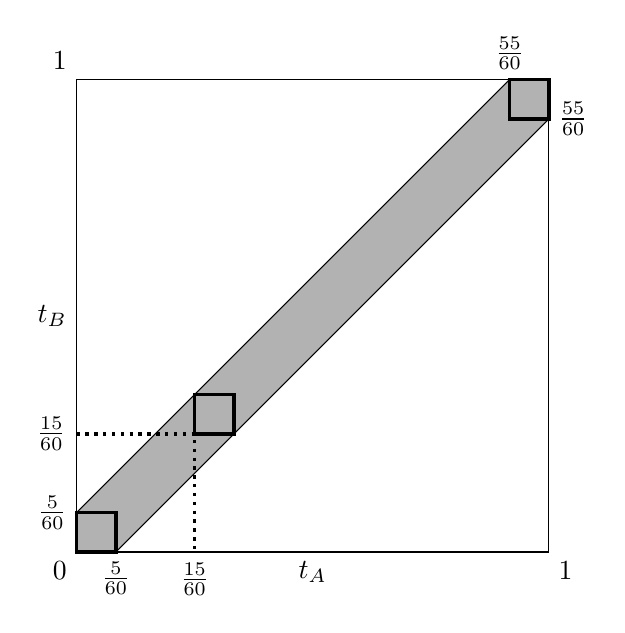
\begin{tikzpicture}
\draw (0,0) -- node[below] {$t_A$} (6,0) -- (6,6) -- (0,6) -- node[left] {$t_B$} cycle;
\node[below left]  at (0,0) {$0$};
\node[below right] at (6,0) {$1$};
\node[above left]  at (0,6) {$1$};
\draw[fill=white!70!black]
  (0,0) -- 
  (.5,0) node[below] {$\frac{5}{60}$} -- 
  (6,5.5) node[right] {$\frac{55}{60}$} --
  (6,6) -- (5.5,6) node[above] {$\frac{55}{60}$} --
  (0,.5) node[left] {$\frac{5}{60}$} -- cycle;
\draw[very thick] (0,0) -- (.5,0) -- (.5,.5) -- (0,.5) -- cycle;
\draw[very thick] (1.5,1.5) -- ++(.5,0) -- ++(0,.5) --
  ++(-.5,0) -- cycle;
\draw[very thick] (5.5,5.5) -- ++(.5,0) -- ++(0,.5) --
  ++(-.5,0) -- cycle;
\draw[very thick,dotted] (0,1.5) node[left] {$\frac{15}{60}$} --
  (1.5,1.5) -- (1.5,0) node[below] {$\frac{15}{60}$};
\end{tikzpicture}
\end{center}
\caption{Times that ensure a meeting between $A$ and $B$}\label{f.duel}
\end{figure}
If $A$ arrives later then $B$ also has to arrive later by the same amount; for example, if $A$ arrives at $15$, $B$ must arrive between $15$ and $20$. Therefore, the meeting will take place during a square of time obtained by moving the small square by $15$ from $(0,0)$ to $(15/60,15/60)$.

The probability that a meeting will occur is the ratio of the area of the graph colored gray to the area of the large square. It is easier to compute the complement which is the area of the white triangles in the upper left and lower right:
\begin{eqnarray*}
P(A,B\;\textsf{meet}) &=& 1- P(A,B\;\textsf{don't meet})\\
&=&1- 2\cdot \left(\frac{1}{2}\cdot \frac{55}{60}\cdot \frac{55}{60}\right)=\frac{23}{144}\approx 0.1597\,.
\end{eqnarray*}

\textbf{Simulation}
\begin{verbatim}
Probability of meeting   = 0.1597
Proportion of meetings   = 0.1549
\end{verbatim}

%%%%%%%%%%%%%%%%%%%%%%%%%%%%%%%%%%%%%%%%%%%%%%%%%%%%%%%%%%%%%

\begin{prob}{Catching the cautious counterfeiter\annotate{S}}

There are $n$ boxes each with $n$ coins and one coin in each box is counterfeit. Draw one coin from each box and test it to determine whether it is counterfeit or not. What is the probability that all the coins that are drawn are are real?

\que{1} Solve for $n=10$.

\que{2} Solve for $n=100$.

\que{3} Solve for arbitrary $n$.

\que{4} What is the limit, if it exists, of the probability as $n$ tends to infinity?
\end{prob}

\solution{}

The draws are independent so the probability is the product of the probabilities for each draw.

\ans{1}
\[
P(\textsf{all real}) = \left(\frac{9}{10}\right)^{10}=0.3487\,.
\]


\ans{2}
\[
P(\textsf{all real}) = \left(\frac{99}{100}\right)^{100}=0.3660\,.
\]

\ans{3}
\[
P(\textsf{all real}) = \left(\frac{n-1}{n}\right)^{n}\,.
\]

\ans{4}
\begin{equation}\label{eq.reciprocal}
\lim_{n\rightarrow\infty}\left(1-\frac{1}{n}\right)^{n}=\frac{1}{e}\approx 0.3679\,.
\end{equation}

This limit can be proved using differential calculus. First we compute the limit of the natural logarithm of the lefthand side of Equation~\ref{eq.reciprocal}:
\[
\lim_{n\rightarrow\infty}\ln \left(1-\frac{1}{n}\right)^{n}=
  \lim_{n\rightarrow\infty}n\ln \left(1-\frac{1}{n}\right)=
  \lim_{n\rightarrow\infty} \disfrac{\ln\left(1-\frac{1}{n}\right)}{1/n}\,.
\]
Taking the limit gives $\ln(1)/0=0/0$ but by l'H\^{o}pital's rule we can replace it by the quotient of the derivatives:
\begin{eqnarray*}
\lim_{n\rightarrow\infty}\ln \left(1-\frac{1}{n}\right)^{n}&=&\lim_{n\rightarrow\infty}\frac{\left(1-\frac{1}{n}\right)^{-1}(-(-n^{-2}))}{-n^{-2}}=-1\\
\lim_{n\rightarrow\infty}\left(1-\frac{1}{n}\right)^{n}&=&e^{-1}\,.
\end{eqnarray*}

\textbf{Simulation}
\begin{verbatim}
For  10 boxes:
Probability of all real = 0.3487
Proportion all real     = 0.3480
For 100 boxes:
Probability of all real = 0.3660
Proportion all real     = 0.3730
For 200 boxes:
Probability of all real = 0.3670
Proportion all real     = 0.3690
\end{verbatim}

%%%%%%%%%%%%%%%%%%%%%%%%%%%%%%%%%%%%%%%%%%%%%%%%%%%%%%%%%%%%%

\begin{prob}{Catching the greedy counterfeiter\annotate{S}}
There are $n$ boxes each with $n$ coins and $m$ coins in each box are counterfeit. Draw one coin from each box and test it to determine whether it is counterfeit or not. What is the probability $P(n,m,r)$ that $r$ of the coins that are drawn are \emph{counterfeit}?

\que{1} Develop a formula for $P(n,m,r)$.

\que{2} Compute $P(20,10,2), P(20,10,8), P(20,5,2), P(20,5,4)$.
\end{prob}

\solution{}

\ans{1}
There are ${n\choose r}$ choices of boxes from which the counterfeit coins can be drawn. From the binomial distribution:
\[
P(n,m,r) = {n \choose r} \left(\frac{m}{n}\right)^r \left(\frac{n-m}{n}\right)^{n-r}\,.
\]

\ans{2}
\begin{eqnarray*}
P(20,10,2) &=& \dischoose{20}{2} \left(\frac{10}{20}\right)^2 \left(\frac{10}{20}\right)^{18}\approx 0.0002\\
P(20,10,8) &=& \dischoose{20}{8} \left(\frac{10}{20}\right)^{8} \left(\frac{10}{20}\right)^{12}\approx 0.1201\\
P(20,5,2)&=&\dischoose{20}{2} \left(\frac{5}{20}\right)^2 \left(\frac{15}{20}\right)^{18}\approx 0.0669\\
P(20,5,4)&=&\dischoose{20}{4} \left(\frac{5}{20}\right)^{4} \left(\frac{15}{20}\right)^{12}\approx 0.1952\,.
\end{eqnarray*}

Mosteller shows that in as $n$ tends to infinity, for fixed $m,r$ the probability is:
\begin{equation}\label{eq.bin-limit}
\lim_{n\rightarrow \infty}P(n,m,r) = \frac{e^{-m}m^r}{r!}\,.
\end{equation}

\textbf{Simulation}
\begin{verbatim}
For 10 bad coins,  2 draws:
Probability of counterfeit  = 0.0002
Proportion counterfeit      = 0.0002
For 10 bad coins,  8 draws:
Probability of counterfeit  = 0.1201
Proportion counterfeit      = 0.1181
For  5 bad coins,  2 draws:
Probability of counterfeit  = 0.0669
Proportion counterfeit      = 0.0688
For  5 bad coins,  4 draws:
Probability of counterfeit  = 0.1897
Proportion counterfeit      = 0.1905
\end{verbatim}

%%%%%%%%%%%%%%%%%%%%%%%%%%%%%%%%%%%%%%%%%%%%%%%%%%%%%%%%%%%%%

\begin{prob}{Moldy gelatin\annotate{S}}

A rectangular plate is divided into $n$ small squares. There are an average of $r$ microbes in each square.

\que{1} Develop a formula for probability that there are exactly $r$ microbes in the $n$ squares.

\que{2} Compute the probability for $n=100,r=3$.

\textbf{Hint:} This problem is similar the Problem~28.

\end{prob}

\solution{}

\ans{1}
Let $p$ be the probability that a single square contains a microbe. (Ignore the possibility that a microbe is partially contained within two or more squares.) $m$, the average number of microbes per square, is the number of squares $n$ times the probability $p$ that a square contains a microbe. $P(n,m,r)$, the probability that there are exactly $r$ microbes in the $n$ squares is given by the binomial distribution:
\[
P(n,m,r) = {n \choose r} \left(\frac{m}{n}\right)^r \left(\frac{n-m}{n}\right)^{n-r}\,.
\]

\ans{2} 
\[
P(10,3,3) = {100 \choose 3} \left(\frac{3}{100}\right)^3 \left(\frac{97}{100}\right)^{97}\approx 0.2275\,.
\]
Equation~\ref{eq.bin-limit} also applies here:
\[
\lim_{n\rightarrow \infty} P(n,3,3) = \frac{e^{-3}\cdot 3^3}{3!}\approx 0.2240\,.
\]
\textbf{Simulation}
\begin{verbatim}
For  20 squares:
Probability of exactly  3 microbes  = 0.2428
Proportion of exactly   3 microbes  = 0.2436
Probability of exactly  5 microbes  = 0.2023
Proportion of exactly   5 microbes  = 0.1954
For 100 squares:
Probability of exactly  3 microbes  = 0.2275
Proportion of exactly   3 microbes  = 0.2247
Probability of exactly  5 microbes  = 0.1800
Proportion of exactly   5 microbes  = 0.1851
\end{verbatim}

%%%%%%%%%%%%%%%%%%%%%%%%%%%%%%%%%%%%%%%%%%%%%%%%%%%%%%%%%%%%%

\refstepcounter{problem} % 30. Evening the sales

%%%%%%%%%%%%%%%%%%%%%%%%%%%%%%%%%%%%%%%%%%%%%%%%%%%%%%%%%%%%%
